\documentclass{article}
\usepackage{xcolor}
\usepackage{ragged2e}
\usepackage{graphicx}
\usepackage{subcaption}
\graphicspath{ {./sdcard/Download/fwc/} }

\begin{document}

\begin{center}
	\color{blue} CHAPTER 7: TRIANGLES
\end{center}
\begin{center}
	\color{blue} EXERCISE 7.3
\end{center}

\begin{enumerate}
	\item $\textbf{ABC}$ is an isosceles triangle with $\textbf{AB=AC}$ and $\textbf{BD}$ and $\textbf{CE}$ are its two medians. Show that $\textbf{BD=CE}$.
	\item In Fig.7.4, $\vec{\textbf{D}}$ and $\vec{\textbf{E}}$ are the points on side $\textbf{BC}$ of a $\triangle \textbf{ABC}$ such that $\textbf{BD=CE}$ and $\textbf{AD=AE}$. Show that $\triangle \textbf{ABD} \cong \triangle \textbf{ACE}$.
\begin{figure}[h]
	\centering
	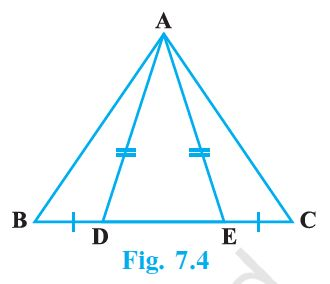
\includegraphics[width=50mm,scale=0.3]{Figure1}
	\caption{}
	\label{image1}
\end{figure}
\item $\textbf{CDE}$ is an equilateral triangle formed on a side $\textbf{CD}$ of a square $\textbf{ABCD}$ (Fig.7.5). Show that $\triangle \textbf{ADE} \cong \triangle \textbf{BCE}$.
\begin{figure}[h]
	\centering
	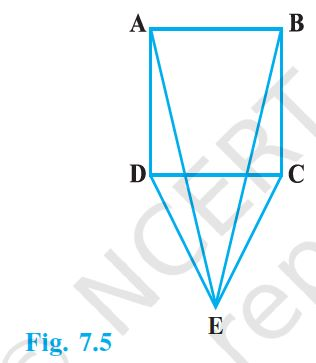
\includegraphics[width=50mm,scale=0.3]{Figure2}
	\caption{}
	\label{image2}
\end{figure}
\item In Fig.7.6, $\textbf{BA} \perp \textbf{AC}$, $\textbf{DE} \perp \textbf{DF}$ such that $\textbf{BA=DE}$ and $\textbf{BF=EC}$. Show that $\triangle \textbf{ABC} \cong \triangle \textbf{DEF}$.
\begin{figure}[h]
	\centering
	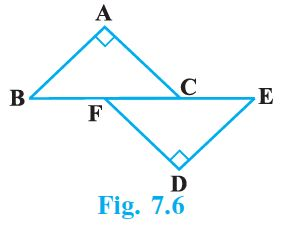
\includegraphics[width=50mm,scale=0.3]{Figure3}
	\caption{}
	\label{image3}
\end{figure}
\item $\vec{\textbf{Q}}$ is a point on the side $\textbf{SR}$ of $\triangle \textbf{PSR}$ such that $\textbf{PQ=PR}$. Prove that $\textbf{PS$>$PQ}$.
\item $\vec{\textbf{S}}$ is any point on side $\textbf{QR}$ of a $\triangle \textbf{PQR}$. Show that $\textbf{PQ+QR+RP$>$2PS}$.
\item $\vec{\textbf{D}}$ is any point on side $\textbf{AC}$ of a $\triangle \textbf{ABC}$ with $\textbf{AB=AC}$. Show that $\textbf{CD$<$BD}$.
\item In Fig.7.7, $\textbf{l} \| \textbf{m}$ an $\vec{\textbf{M}}$ is the mid-point of a line segment $\textbf{AB}$. Show that $\vec{\textbf{M}}$ is also the mid-point of any line segment $\textbf{CD}$, having its end points on $\textbf{l}$ and $\textbf{m}$, respectively.
\begin{figure}[h]
	\centering
	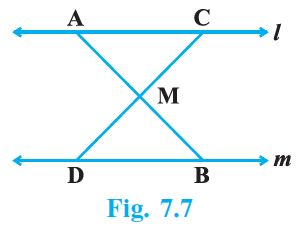
\includegraphics[width=50mm,scale=0.3]{Figure4}
	\caption{}
	\label{image4}
\end{figure}
\item Bisectors of the $\angle \textbf{B}$ and $\angle \textbf{C}$ of an isosceles triangle with $\textbf{AB=AC}$ intersect each other at $\vec{\textbf{O}}$. $\textbf{BO}$ is produced to a point $\textbf{M}$. Prove that $\angle \textbf{MOC}= \angle \textbf{ABC}$.
\item Bisectors of the $\angle \textbf{B}$ and $\angle \textbf{C}$ of an isosceles triangle $\textbf{ABC}$ with $\textbf{AB=AC}$ intersect each other at $\vec{\textbf{O}}$. Show that the external angle adjacent to $\angle \textbf{ABC}$ is equal to $\angle \textbf{BOC}$.
\pagebreak
\item In Fig.7.8, $\textbf{AD}$ is the bisector of $\angle \textbf{BAC}$. Prove that $\textbf{AB$>$BD}$.
	\begin{figure}[h]
	\centering
	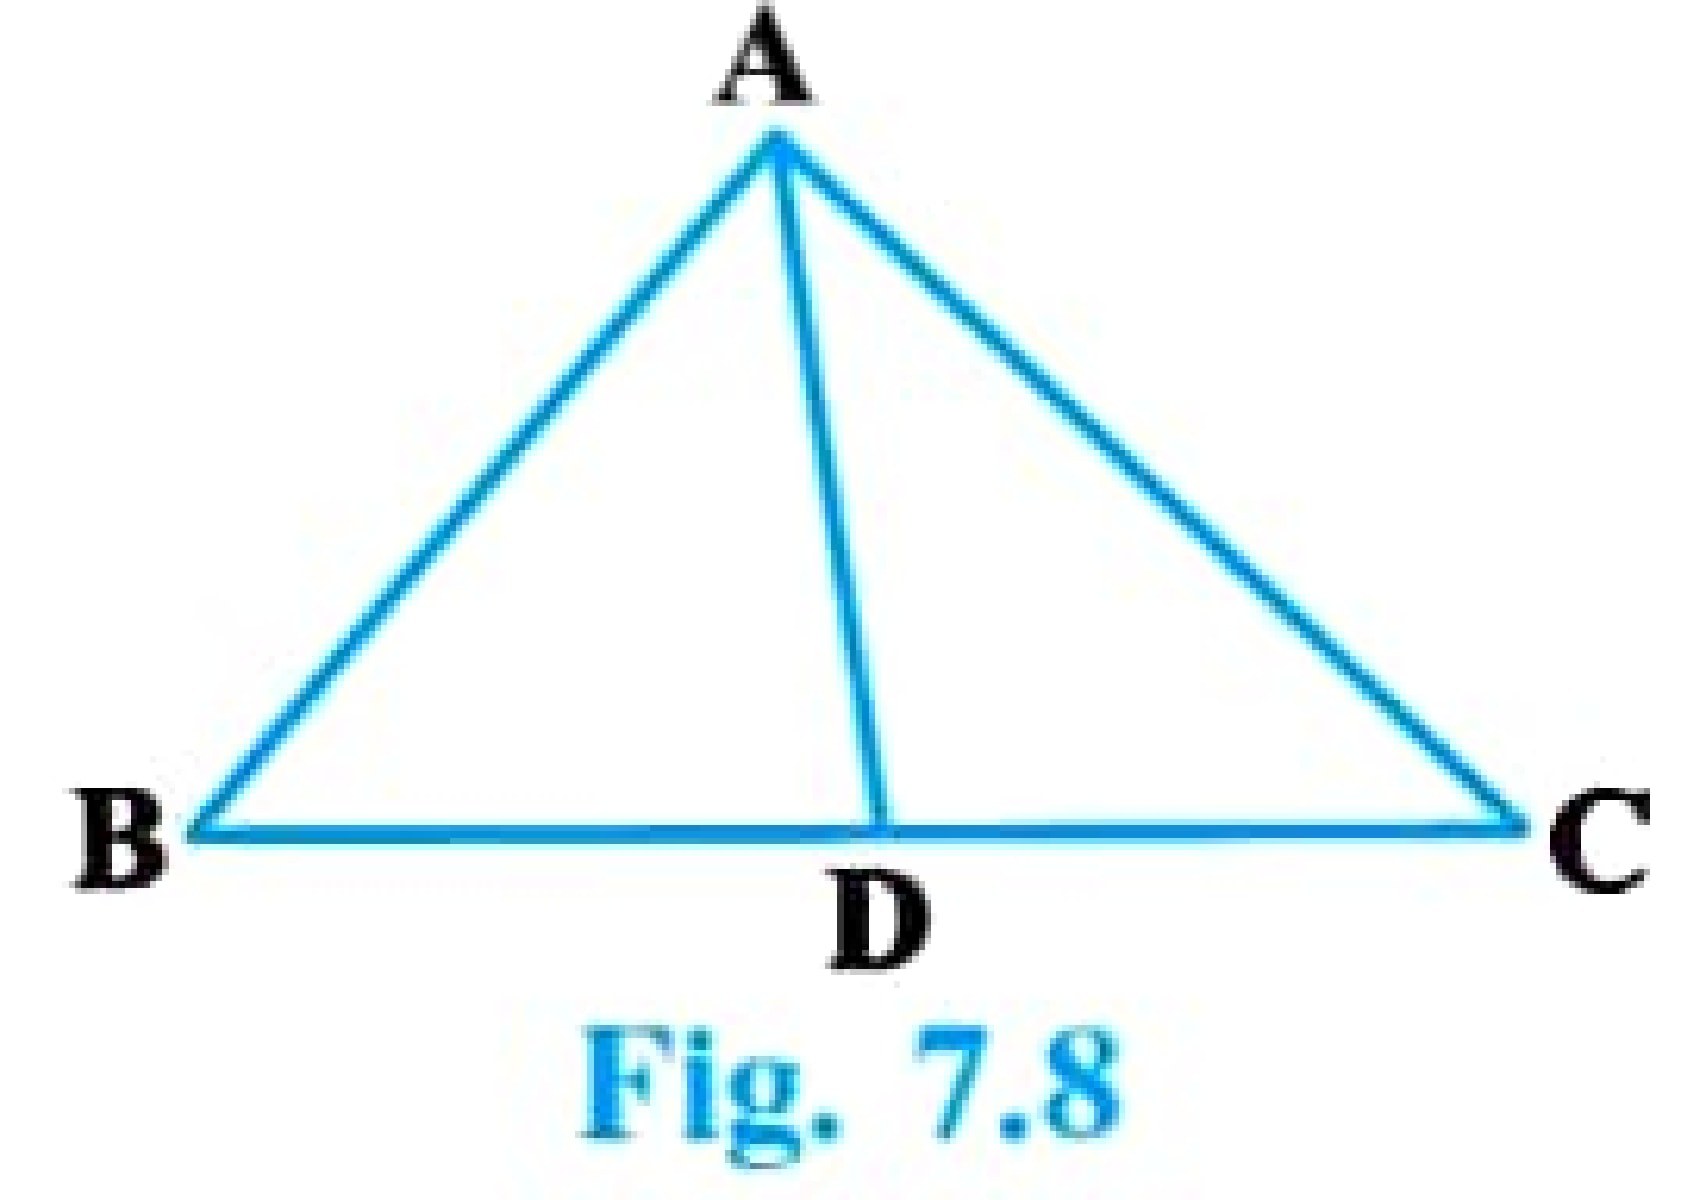
\includegraphics[width=50mm,scale=0.08]{Figure5}
	\caption{}
	\label{image5}
\end{figure}
\end{enumerate}
\end{document}
